% ============================================================
%  Module 4 — Marx and the Machinery Question
%  From Smith to Simulation · University of Edinburgh
% ============================================================
\documentclass[aspectratio=169, 10pt]{beamer}
\usetheme{metropolis}

% --- Edinburgh colours ----------------------------------------
\definecolor{UoERed}{HTML}{7A2318}
\definecolor{UoEGold}{HTML}{B8860B}
\definecolor{CodeBG}{HTML}{F7F3ED}
\definecolor{CodeFrame}{HTML}{D5C9B1}

\setbeamercolor{palette primary}{bg=UoERed, fg=white}
\setbeamercolor{frametitle}{bg=UoERed, fg=white}
\setbeamercolor{title separator}{fg=UoEGold}
\setbeamercolor{progress bar}{fg=UoEGold, bg=UoEGold!20}
\setbeamercolor{alerted text}{fg=UoERed}
\setbeamercolor{block title}{bg=UoERed!15, fg=UoERed}
\setbeamercolor{block body}{bg=UoERed!5}

% --- Packages -------------------------------------------------
\usepackage[T1]{fontenc}
\usepackage{lmodern}
\usepackage{amsmath, amssymb, mathtools}
\usepackage{listings}
\usepackage{graphicx, booktabs}
\usepackage{tikz}
\usetikzlibrary{arrows.meta, positioning, calc, decorations.pathreplacing}
\usepackage{hyperref}
\hypersetup{colorlinks=true, linkcolor=UoERed, urlcolor=UoERed!70!black}
\setbeamertemplate{navigation symbols}{}

\lstset{
  language=Python,
  basicstyle=\ttfamily\scriptsize,
  keywordstyle=\color{UoERed}\bfseries,
  commentstyle=\color{gray}\itshape,
  stringstyle=\color{UoEGold},
  backgroundcolor=\color{CodeBG},
  frame=single,
  rulecolor=\color{CodeFrame},
  numbers=none,
  breaklines=true,
  showstringspaces=false,
  tabsize=4,
  xleftmargin=4pt, xrightmargin=4pt,
  aboveskip=6pt, belowskip=4pt,
}

% Section title pages
\AtBeginSection[]{
  \begin{frame}
    \vfill\centering
    \usebeamerfont{title}\insertsectionhead\par
    \vfill
  \end{frame}
}

% ---- Title ---------------------------------------------------
\title{Module 4 --- Marx and the Machinery Question}
\subtitle{Capital, Surplus Value, and the Labour Share}
\author{Dr Juan Zurita}
\institute{From Smith to Simulation\\
The University of Edinburgh~$\cdot$~School of Economics}
\date{}

\begin{document}

% =============================================================
\maketitle
% =============================================================

% -------------------------------------------------------------
\section{Part I --- The History}
% -------------------------------------------------------------

\begin{frame}{The Dark Side of the Pin Factory}
\begin{columns}[T]
\column{0.55\textwidth}
\begin{itemize}
  \item Adam Smith marvelled at the pin factory's productivity.
  \item But by the 1840s, the Industrial Revolution raised an
        uncomfortable question: \alert{who benefits?}
  \item Factories produced more than ever, yet workers laboured
        14-hour days in dangerous conditions.
  \item Children as young as five worked in coal mines.
  \item Meanwhile, factory owners grew spectacularly rich.
\end{itemize}
\column{0.4\textwidth}
\begin{block}{The Gap Widens}
The gap between capital and labour had never been wider.
This was the world that \textbf{Karl Marx} (1818--1883)
set out to explain.
\end{block}
\end{columns}
\end{frame}

\begin{frame}{Karl Marx and Friedrich Engels}
\begin{columns}[T]
\column{0.55\textwidth}
\begin{itemize}
  \item \textbf{Karl Marx} (1818--1883): German philosopher,
        economist, and revolutionary.
  \item Collaborated with \textbf{Friedrich Engels}, son of a
        Manchester factory owner who witnessed working conditions
        first-hand.
  \item \textit{The Communist Manifesto} (1848): ``The history
        of all hitherto existing society is the history of
        class struggles.''
  \item \textit{Capital} (Das Kapital, 1867): a massive analysis
        of how capitalism works --- and why, Marx argued, it
        would eventually \alert{destroy itself}.
\end{itemize}
\column{0.4\textwidth}
\begin{block}{Method}
Writing from the reading room of the British Museum, Marx
combined Hegelian philosophy, Ricardo's economics, and
detailed empirical study of factory reports.
\end{block}
\end{columns}
\end{frame}

\begin{frame}{Surplus Value}
\begin{center}
\textit{``The essential difference between the various economic forms
of society \ldots\ lies only in the mode in which this surplus labour
is in each case extracted from the actual producer, the labourer.''}\\[4pt]
--- Karl Marx, \textit{Capital}, Vol.~I, Ch.~9
\end{center}
\vspace{0.8em}
\begin{columns}[T]
\column{0.48\textwidth}
\begin{block}{Labour Theory of Value}
The value of a good comes from the labour required to produce it.
A chair is worth more than a stick because more labour went into it.
\end{block}
\column{0.48\textwidth}
\begin{block}{Surplus Value}
Workers produce more value than they receive in wages. A worker
produces \pounds 10/hour but earns \pounds 3. The remaining
\alert{\pounds 7} is \textbf{surplus value}, captured as profit.
\end{block}
\end{columns}
\end{frame}

\begin{frame}{The Machinery Question}
\begin{center}
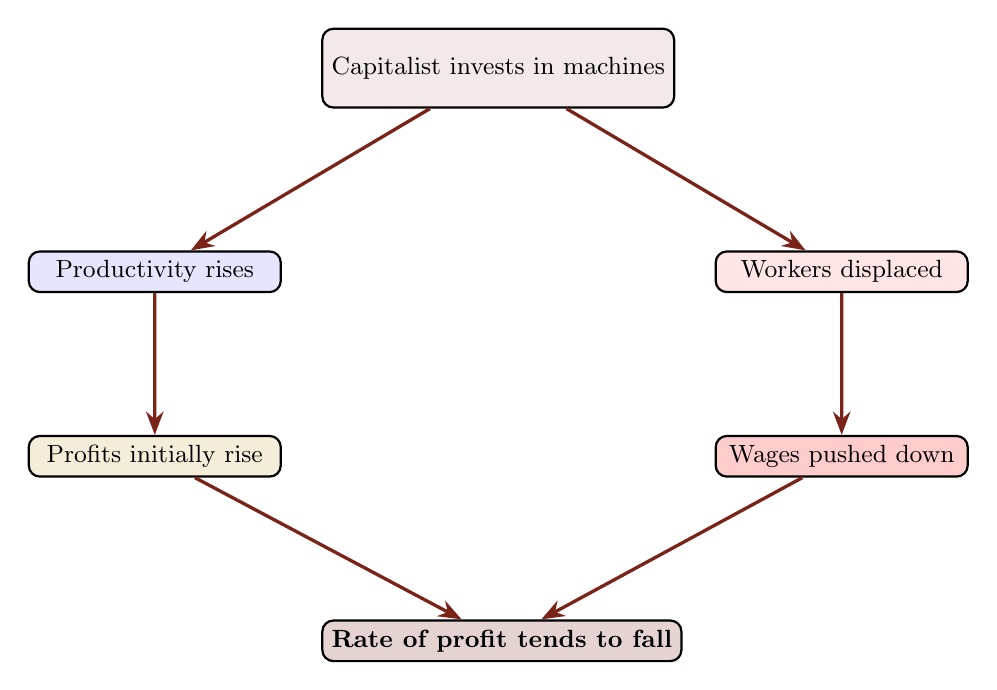
\begin{tikzpicture}[>=Stealth, thick, scale=0.85]
  \node[draw, rounded corners, fill=UoERed!10, minimum width=3.8cm,
        minimum height=1cm, font=\small] (cap)
    {Capitalist invests in machines};
  \node[below left=1.8cm and 0.5cm of cap, draw, rounded corners,
        fill=blue!10, minimum width=3.2cm, font=\small] (prod)
    {Productivity rises};
  \node[below right=1.8cm and 0.5cm of cap, draw, rounded corners,
        fill=red!10, minimum width=3.2cm, font=\small] (disp)
    {Workers displaced};
  \node[below=1.8cm of prod, draw, rounded corners, fill=UoEGold!15,
        minimum width=3.2cm, font=\small] (profit)
    {Profits initially rise};
  \node[below=1.8cm of disp, draw, rounded corners, fill=red!20,
        minimum width=3.2cm, font=\small] (wages)
    {Wages pushed down};
  \node[below right=1.8cm and 0.5cm of profit, draw, rounded corners,
        fill=UoERed!20, minimum width=4cm, font=\small\bfseries] (fall)
    {Rate of profit tends to fall};

  \draw[->, line width=1.2pt, UoERed] (cap) -- (prod);
  \draw[->, line width=1.2pt, UoERed] (cap) -- (disp);
  \draw[->, line width=1.2pt, UoERed] (prod) -- (profit);
  \draw[->, line width=1.2pt, UoERed] (disp) -- (wages);
  \draw[->, line width=1.2pt, UoERed] (profit) -- (fall);
  \draw[->, line width=1.2pt, UoERed] (wages) -- (fall);
\end{tikzpicture}
\end{center}
\vspace{0.3em}
Marx called the rising capital-to-labour ratio the
\textbf{organic composition of capital} rising.
\end{frame}

\begin{frame}{The Machinery Question in the 21st Century}
Marx's question --- \textit{does technology help or hurt workers?}
--- is more relevant today than ever.
\vspace{0.5em}
\begin{itemize}
  \item Since the 1980s, the \textbf{labour share of income} has been
        declining across developed economies.
  \item Automation, globalisation, and now \alert{artificial intelligence}
        raise the same concerns Marx identified in 1867.
  \item We cannot resolve this debate in one module, but we can build a
        model that \textbf{formalises the question} and lets us explore
        the forces at work.
\end{itemize}
\vspace{0.5em}
\begin{alertblock}{Central Question}
Under what conditions does capital accumulation reduce workers'
share of income --- and under what conditions does it raise
their wages?
\end{alertblock}
\end{frame}

\begin{frame}{Edinburgh Connection}
\begin{columns}[T]
\column{0.55\textwidth}
Edinburgh's own Industrial Revolution was the backdrop for these
debates:
\vspace{0.3em}
\begin{itemize}
  \item The city was once Britain's \textbf{second-largest brewing centre}.
  \item Expansion of \textbf{printing} and \textbf{engineering} industries.
  \item The \textit{Edinburgh Review} (founded 1802) was one of the key
        journals where political economists debated the effects of
        machinery on employment.
\end{itemize}
\column{0.4\textwidth}
\begin{block}{The Edinburgh Review}
Founded by Sydney Smith, Francis Jeffrey, and Henry Brougham,
the \textit{Edinburgh Review} shaped public debate on
industrialisation, free trade, and the condition of the
working class for over a century.
\end{block}
\end{columns}
\end{frame}

% -------------------------------------------------------------
\section{Part II --- The Computation}
% -------------------------------------------------------------

\begin{frame}[fragile]{Setting Up}
\begin{lstlisting}
import numpy as np
import matplotlib.pyplot as plt
\end{lstlisting}
\vspace{0.5em}
\begin{itemize}
  \item \texttt{numpy} --- numerical arrays and operations
  \item \texttt{matplotlib} --- plotting
\end{itemize}
\vspace{0.5em}
Today we model how output is \textbf{divided} between capital and
labour --- and what happens when capitalists accumulate more and
more machines.
\end{frame}

\begin{frame}{The Cobb-Douglas Production Function}
We model output using a \textbf{Cobb-Douglas production function}:
\vspace{0.3em}
\[
  Y = A \cdot K^{\alpha} \cdot L^{1-\alpha}
\]
\vspace{0.3em}
\begin{description}
  \item[$K$] Capital (machines, factories)
  \item[$L$] Labour (workers)
  \item[$A$] Total factor productivity
  \item[$\alpha \in (0,1)$] The \alert{capital share} --- the fraction
        of income going to capital owners
\end{description}
\vspace{0.5em}
Key property: \textbf{constant returns to scale}.
Doubling both $K$ and $L$ exactly doubles $Y$.
\end{frame}

\begin{frame}{Factor Payments: Who Gets What?}
In competitive markets, factors are paid their \textbf{marginal products}:
\vspace{0.3em}
\begin{align*}
  \text{Wage:} \quad w &= \text{MPL} = (1-\alpha)\,\frac{Y}{L}
      = (1-\alpha)\,A\,K^{\alpha}\,L^{-\alpha} \\[8pt]
  \text{Rental rate:} \quad r &= \text{MPK} = \alpha\,\frac{Y}{K}
      = \alpha\,A\,K^{\alpha-1}\,L^{1-\alpha}
\end{align*}
\vspace{0.3em}
\begin{columns}[T]
\column{0.48\textwidth}
\begin{block}{Labour Share}
  $\displaystyle \frac{wL}{Y} = 1 - \alpha$
\end{block}
\column{0.48\textwidth}
\begin{block}{Capital Share}
  $\displaystyle \frac{rK}{Y} = \alpha$
\end{block}
\end{columns}
\vspace{0.5em}
Under Cobb-Douglas, these shares are \alert{constant} ---
a result roughly true from 1950 to 1980, but since broken down.
\end{frame}

\begin{frame}[fragile]{Defining the Production Function in Python}
\begin{lstlisting}
# Parameters
A = 1.0
alpha = 0.33    # capital share
L = 100         # fixed labour supply

def output(K, L=L, A=A, alpha=alpha):
    return A * K**alpha * L**(1 - alpha)

def wage(K, L=L, A=A, alpha=alpha):
    return (1 - alpha) * A * K**alpha * L**(-alpha)

def rental_rate(K, L=L, A=A, alpha=alpha):
    return alpha * A * K**(alpha - 1) * L**(1 - alpha)
\end{lstlisting}
\vspace{0.3em}
As capital accumulates:
\begin{itemize}
  \item Output rises (but with diminishing returns)
  \item Wages \textbf{rise} (more capital per worker)
  \item Return on capital \textbf{falls} (diminishing returns)
  \item Labour share stays constant at $1-\alpha = 67\%$
\end{itemize}
\end{frame}

\begin{frame}{Output and Factor Prices as Capital Grows}
\begin{center}
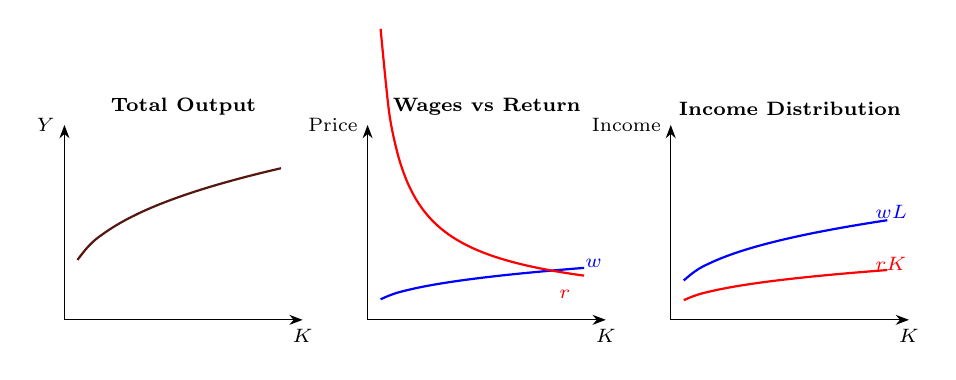
\begin{tikzpicture}[scale=0.55, >=Stealth]
  % --- Panel 1: Output ---
  \begin{scope}[xshift=0cm]
    \draw[->] (0,0) -- (5.5,0) node[below, font=\scriptsize] {$K$};
    \draw[->] (0,0) -- (0,4.5) node[left, font=\scriptsize] {$Y$};
    \draw[thick, UoERed!70!black] plot[smooth, domain=0.3:5]
      (\x, {3.5*(\x/5)^0.33});
    \node[above, font=\scriptsize\bfseries] at (2.75, 4.5) {Total Output};
  \end{scope}
  % --- Panel 2: Factor Prices ---
  \begin{scope}[xshift=7cm]
    \draw[->] (0,0) -- (5.5,0) node[below, font=\scriptsize] {$K$};
    \draw[->] (0,0) -- (0,4.5) node[left, font=\scriptsize] {Price};
    \draw[thick, blue] plot[smooth, domain=0.3:5]
      (\x, {1.2*(\x/5)^0.33});
    \draw[thick, red] plot[smooth, domain=0.3:5]
      (\x, {3.0*(\x)^(-0.67)});
    \node[right, font=\scriptsize, blue] at (4.8, 1.3) {$w$};
    \node[right, font=\scriptsize, red] at (4.2, 0.6) {$r$};
    \node[above, font=\scriptsize\bfseries] at (2.75, 4.5) {Wages vs Return};
  \end{scope}
  % --- Panel 3: Income Distribution ---
  \begin{scope}[xshift=14cm]
    \draw[->] (0,0) -- (5.5,0) node[below, font=\scriptsize] {$K$};
    \draw[->] (0,0) -- (0,4.5) node[left, font=\scriptsize] {Income};
    \draw[thick, blue] plot[smooth, domain=0.3:5]
      (\x, {2.3*(\x/5)^0.33});
    \draw[thick, red] plot[smooth, domain=0.3:5]
      (\x, {1.15*(\x/5)^0.33});
    \node[right, font=\scriptsize, blue] at (4.5, 2.5) {$wL$};
    \node[right, font=\scriptsize, red] at (4.5, 1.3) {$rK$};
    \node[above, font=\scriptsize\bfseries] at (2.75, 4.5) {Income Distribution};
  \end{scope}
\end{tikzpicture}
\end{center}
\vspace{0.3em}
Under Cobb-Douglas, wages \textbf{rise} with capital but the
\textbf{shares} remain fixed: $wL/Y = 1-\alpha$, $rK/Y = \alpha$.
\end{frame}

\begin{frame}[fragile]{Plotting Factor Prices in Python}
\begin{lstlisting}
K_range = np.linspace(10, 500, 200)
Y = output(K_range)
total_wages = wage(K_range) * L
total_profits = rental_rate(K_range) * K_range

fig, axes = plt.subplots(1, 3, figsize=(15, 4.5))

axes[0].plot(K_range, Y, color='seagreen', linewidth=2)
axes[0].set_title('Total Output')

axes[1].plot(K_range, wage(K_range), label='Wage per worker')
axes[1].plot(K_range, rental_rate(K_range), label='Return on capital')
axes[1].legend()

axes[2].plot(K_range, total_wages, label='Total wages (wL)')
axes[2].plot(K_range, total_profits, label='Total profits (rK)')
axes[2].legend()
\end{lstlisting}
\end{frame}

\begin{frame}{Capital Accumulation Dynamics}
Marx was interested in the \textit{dynamics} of capitalism.
Capitalists reinvest their profits, accumulating more and more capital:
\vspace{0.5em}
\[
  K_{t+1} = (1 - \delta)\,K_t + s \cdot r_t \cdot K_t
\]
\vspace{0.3em}
\begin{description}
  \item[$\delta$] Depreciation rate (machines wear out)
  \item[$s$] Fraction of profits that capitalists reinvest
  \item[$r_t \cdot K_t$] Total profits in period $t$
\end{description}
\vspace{0.5em}
\begin{alertblock}{Steady State}
In the long run, $K$ converges to a steady state where investment
equals depreciation: $s \cdot r \cdot K = \delta \cdot K$, giving
$r_{\text{ss}} = \delta / s$.
\end{alertblock}
\end{frame}

\begin{frame}[fragile]{Simulating Capital Accumulation}
\begin{lstlisting}
T = 200
delta = 0.05    # depreciation rate
s = 0.80        # reinvestment rate
K0 = 50         # initial capital

def simulate_accumulation(K0, L, A, alpha, delta, s, T):
    K = np.empty(T)
    K[0] = K0
    Y_t, w_t, r_t = [np.empty(T) for _ in range(3)]
    for t in range(T):
        Y_t[t] = output(K[t], L, A, alpha)
        w_t[t] = wage(K[t], L, A, alpha)
        r_t[t] = rental_rate(K[t], L, A, alpha)
        if t < T - 1:
            K[t+1] = (1 - delta)*K[t] + s*r_t[t]*K[t]
    return K, Y_t, w_t, r_t

K_sim, Y_sim, w_sim, r_sim = simulate_accumulation(
    K0, L, A, alpha, delta, s, T)
\end{lstlisting}
\end{frame}

\begin{frame}{Convergence: Capital and the Rate of Profit}
\begin{center}
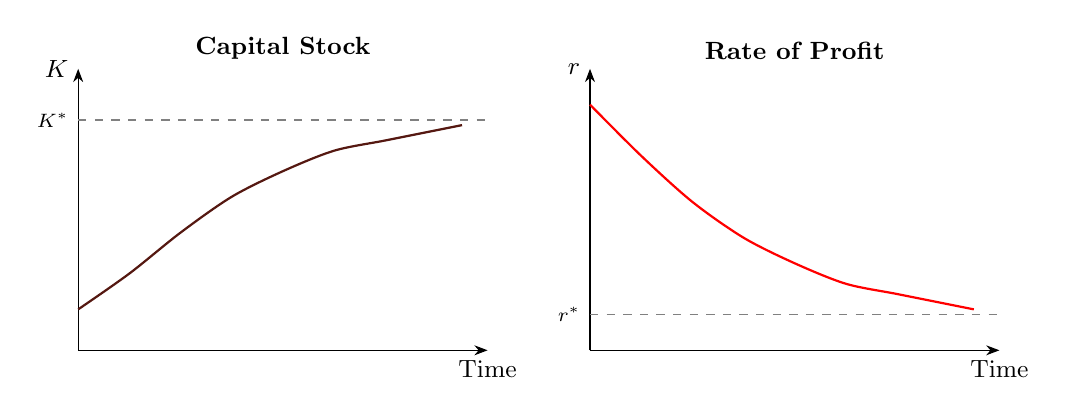
\begin{tikzpicture}[scale=0.65, >=Stealth]
  % --- Panel 1: Capital ---
  \begin{scope}[xshift=0cm]
    \draw[->] (0,0) -- (8,0) node[below, font=\small] {Time};
    \draw[->] (0,0) -- (0,5.5) node[left, font=\small] {$K$};
    \draw[thick, UoERed!70!black] plot[smooth] coordinates
      {(0,0.8) (1,1.5) (2,2.3) (3,3.0) (4,3.5) (5,3.9) (6,4.1) (7,4.3) (7.5,4.4)};
    \draw[dashed, gray] (0, 4.5) -- (8, 4.5);
    \node[left, font=\scriptsize] at (0, 4.5) {$K^*$};
    \node[above, font=\small\bfseries] at (4, 5.5) {Capital Stock};
  \end{scope}
  % --- Panel 2: Rate of Profit ---
  \begin{scope}[xshift=10cm]
    \draw[->] (0,0) -- (8,0) node[below, font=\small] {Time};
    \draw[->] (0,0) -- (0,5.5) node[left, font=\small] {$r$};
    \draw[thick, red] plot[smooth] coordinates
      {(0,4.8) (1,3.8) (2,2.9) (3,2.2) (4,1.7) (5,1.3) (6,1.1) (7,0.9) (7.5,0.8)};
    \draw[dashed, gray] (0, 0.7) -- (8, 0.7);
    \node[left, font=\scriptsize] at (0, 0.7) {$r^*$};
    \node[above, font=\small\bfseries] at (4, 5.5) {Rate of Profit};
  \end{scope}
\end{tikzpicture}
\end{center}
\vspace{0.5em}
As capital accumulates, \textbf{diminishing returns} drive down the
rate of profit --- exactly Marx's ``tendency of the rate of profit
to fall.''\\[4pt]
But wages \textbf{rise}: more capital per worker raises productivity.
\end{frame}

\begin{frame}{Marx's Falling Rate of Profit}
\begin{columns}[T]
\column{0.55\textwidth}
\begin{itemize}
  \item Marx predicted that as capitalists invest, the return on each
        additional unit of capital declines.
  \item In our model: $r = \alpha A K^{\alpha - 1} L^{1-\alpha}$.
        As $K \to \infty$, $r \to 0$.
  \item At steady state: $r_{\text{ss}} = \delta / s$.
  \item With $\delta = 0.05$, $s = 0.80$: $r_{\text{ss}} = 6.25\%$.
\end{itemize}
\column{0.4\textwidth}
\begin{block}{What Marx Missed}
Sustained \textbf{technological progress} ($A$ rising) can offset
diminishing returns and prevent the profit rate from collapsing.
Marx did not anticipate continuous innovation.
\end{block}
\end{columns}
\vspace{0.5em}
\begin{alertblock}{Key Insight}
Diminishing returns alone push $r$ down, but productivity growth
can \textbf{counteract} this tendency indefinitely.
\end{alertblock}
\end{frame}

\begin{frame}{Beyond Cobb-Douglas: The CES Production Function}
The Cobb-Douglas gives a \textbf{constant} labour share --- which
does not match post-1980 data. We need a more flexible model:
\vspace{0.3em}
\[
  Y = A \left[\alpha\,K^{\frac{\sigma-1}{\sigma}}
    + (1-\alpha)\,L^{\frac{\sigma-1}{\sigma}}
  \right]^{\frac{\sigma}{\sigma-1}}
\]
\vspace{0.3em}
The parameter $\sigma$ is the \textbf{elasticity of substitution}
--- how easily capital can replace labour.
\vspace{0.5em}
\begin{columns}[T]
\column{0.32\textwidth}
\begin{block}{$\sigma = 1$}
Cobb-Douglas.\\
Labour share constant.
\end{block}
\column{0.32\textwidth}
\begin{block}{$\sigma > 1$}
Easy to substitute.\\
Labour share \alert{falls}
as $K$ grows.
\end{block}
\column{0.32\textwidth}
\begin{block}{$\sigma < 1$}
Complements.\\
Labour share \textbf{rises}
as $K$ grows.
\end{block}
\end{columns}
\end{frame}

\begin{frame}[fragile]{CES Production Function in Python}
\begin{lstlisting}
def ces_output(K, L, A, alpha, sigma):
    """CES production function."""
    rho = (sigma - 1) / sigma
    return A * (alpha * K**rho + (1 - alpha) * L**rho)**(1/rho)

def ces_labour_share(K, L, A, alpha, sigma):
    """Labour share under CES production."""
    rho = (sigma - 1) / sigma
    Y = ces_output(K, L, A, alpha, sigma)
    inner = alpha * K**rho + (1 - alpha) * L**rho
    MPL = A * (1 - alpha) * L**(rho - 1) * inner**(1/rho - 1)
    return MPL * L / Y
\end{lstlisting}
\vspace{0.3em}
The key idea: when $\sigma > 1$ and $K$ rises, the marginal product of
labour falls \textit{faster} than the capital--labour ratio rises,
so workers' share of income \textbf{declines}.
\end{frame}

\begin{frame}{Labour Share Under Different Elasticities}
\begin{center}
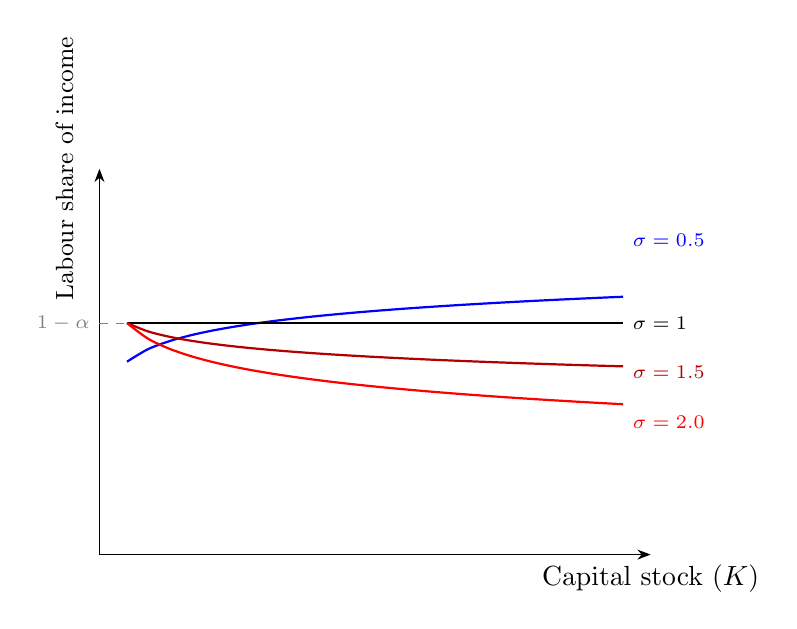
\begin{tikzpicture}[scale=0.7, >=Stealth]
  \draw[->] (0,0) -- (10,0) node[below] {Capital stock ($K$)};
  \draw[->] (0,0) -- (0,7) node[left, rotate=90, anchor=south,
    yshift=6pt, font=\small] {Labour share of income};

  % sigma = 0.5 (complements): share rises
  \draw[thick, blue] plot[smooth, domain=0.5:9.5]
    (\x, {3.5 + 1.2*ln(\x/0.5)/3});
  \node[right, font=\scriptsize, blue] at (9.5, 5.7)
    {$\sigma = 0.5$};

  % sigma = 1 (Cobb-Douglas): constant
  \draw[thick, black] (0.5, 4.2) -- (9.5, 4.2);
  \node[right, font=\scriptsize] at (9.5, 4.2)
    {$\sigma = 1$};

  % sigma = 1.5 (substitutes): share falls
  \draw[thick, red!70!black] plot[smooth, domain=0.5:9.5]
    (\x, {4.2 - 0.8*ln(\x/0.5)/3});
  \node[right, font=\scriptsize, red!70!black] at (9.5, 3.3)
    {$\sigma = 1.5$};

  % sigma = 2 (easy substitution): share falls faster
  \draw[thick, red] plot[smooth, domain=0.5:9.5]
    (\x, {4.2 - 1.5*ln(\x/0.5)/3});
  \node[right, font=\scriptsize, red] at (9.5, 2.4)
    {$\sigma = 2.0$};

  % Annotation
  \draw[dashed, gray] (0, 4.2) -- (0.5, 4.2);
  \node[left, font=\scriptsize, gray] at (0, 4.2) {$1-\alpha$};
\end{tikzpicture}
\end{center}
\vspace{0.3em}
When $\sigma > 1$, \alert{capital accumulation reduces the labour share}
--- exactly what Marx predicted and what we observe since 1980.
\end{frame}

\begin{frame}[fragile]{Computing Labour Shares for Different $\sigma$}
\begin{lstlisting}
K_range = np.linspace(50, 1000, 200)

fig, ax = plt.subplots(figsize=(9, 5))

for sigma, color, ls in [
        (0.5, 'steelblue', 'Complements'),
        (1.01, 'black', 'Cobb-Douglas'),
        (1.5, 'coral', 'Substitutes'),
        (2.0, 'red', 'Easy substitution')]:
    shares = [ces_labour_share(K, L, A, 0.33, sigma)
              for K in K_range]
    ax.plot(K_range, shares, color=color, linewidth=2,
            label=f'{ls} (sigma={sigma})')

ax.set_xlabel('Capital stock (K)')
ax.set_ylabel('Labour share of income')
ax.legend()
ax.set_ylim(0, 1)
\end{lstlisting}
\vspace{0.3em}
Recent estimates put $\sigma$ between 1.2 and 1.6 for the US economy.
\end{frame}

\begin{frame}{US Labour Share, 1950--2020}
\begin{center}
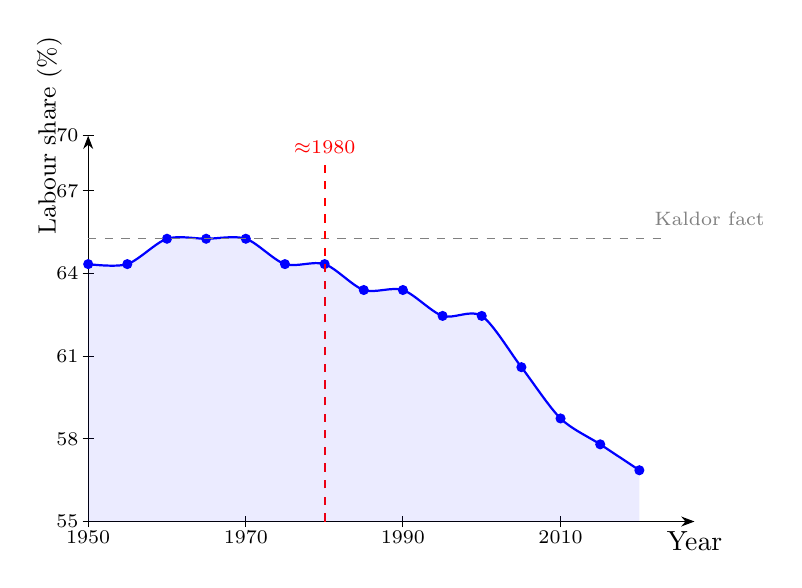
\begin{tikzpicture}[scale=0.7, >=Stealth]
  % Axes
  \draw[->] (0,0) -- (11,0) node[below] {Year};
  \draw[->] (0,0) -- (0,7) node[left, rotate=90, anchor=south,
    yshift=6pt, font=\small] {Labour share (\%)};

  % Y-axis labels (55 to 70)
  \foreach \y/\lab in {0/55, 1.5/58, 3/61, 4.5/64, 6/67, 7/70} {
    \node[left, font=\scriptsize] at (0, \y) {\lab};
    \draw (-0.1, \y) -- (0.1, \y);
  }

  % X-axis labels
  \foreach \x/\lab in {0/1950, 2.86/1970, 5.71/1990, 8.57/2010} {
    \node[below, font=\scriptsize] at (\x, 0) {\lab};
    \draw (\x, -0.1) -- (\x, 0.1);
  }

  % Data points (scaled: x = (year-1950)/7, y = (share-55)/15 * 7)
  % 1950: 65 -> (0, 4.67)   1960: 66 -> (1.43, 5.13)
  % 1970: 66 -> (2.86, 5.13) 1980: 65 -> (4.29, 4.67)
  % 1990: 64 -> (5.71, 4.2)  2000: 63 -> (7.14, 3.73)
  % 2010: 59 -> (8.57, 1.87) 2020: 57 -> (10, 0.93)
  \draw[thick, blue, mark=*] plot[smooth] coordinates
    {(0, 4.67) (0.71, 4.67) (1.43, 5.13) (2.14, 5.13)
     (2.86, 5.13) (3.57, 4.67) (4.29, 4.67)
     (5.0, 4.2) (5.71, 4.2) (6.43, 3.73)
     (7.14, 3.73) (7.86, 2.8) (8.57, 1.87)
     (9.29, 1.4) (10, 0.93)};

  % Kaldor fact line
  \draw[dashed, gray] (0, 5.13) -- (10.5, 5.13);
  \node[right, font=\scriptsize, gray] at (10.1, 5.5) {Kaldor fact};

  % 1980 break line
  \draw[dashed, red, thick] (4.29, 0) -- (4.29, 6.5);
  \node[above, font=\scriptsize, red] at (4.29, 6.5) {$\approx$1980};

  % Fill
  \fill[blue, opacity=0.08] plot[smooth] coordinates
    {(0, 4.67) (0.71, 4.67) (1.43, 5.13) (2.14, 5.13)
     (2.86, 5.13) (3.57, 4.67) (4.29, 4.67)
     (5.0, 4.2) (5.71, 4.2) (6.43, 3.73)
     (7.14, 3.73) (7.86, 2.8) (8.57, 1.87)
     (9.29, 1.4) (10, 0.93)}
    -- (10, 0) -- (0, 0) -- cycle;
\end{tikzpicture}
\end{center}
\vspace{0.3em}
For decades, the labour share was $\approx 66\%$ --- a ``Kaldor fact.''
Since $\approx$1980, it has declined by nearly 10 percentage points.
\end{frame}

\begin{frame}[fragile]{Plotting the Labour Share Data}
\begin{lstlisting}
# Stylised US labour share data
# (based on BLS and Karabarbounis & Neiman 2014)
years = np.array([1950, 1955, 1960, 1965, 1970, 1975, 1980,
                   1985, 1990, 1995, 2000, 2005, 2010, 2015, 2020])
labour_share_us = np.array([0.65, 0.65, 0.66, 0.66, 0.66, 0.65,
    0.65, 0.64, 0.64, 0.63, 0.63, 0.61, 0.59, 0.58, 0.57])

fig, ax = plt.subplots(figsize=(9, 5))
ax.plot(years, labour_share_us*100, 'o-', linewidth=2)
ax.axvline(1980, color='red', linestyle='--', alpha=0.4,
           label='c. 1980: trend break')
ax.axhline(66, color='gray', linestyle=':', alpha=0.5,
           label='"Kaldor fact"')
ax.set_title('US Labour Share of Income, 1950-2020')
ax.legend()
\end{lstlisting}
\vspace{0.3em}
Marx might say: ``I told you so.''
\end{frame}

% -------------------------------------------------------------
\section{Part III --- Exercises \& Discussion}
% -------------------------------------------------------------

\begin{frame}{Exercise 1: Marx's Falling Rate of Profit}
\textbf{(a)} Simulate capital accumulation for 300 periods using
Cobb-Douglas ($\alpha=0.33$, $L=100$, $A=1$, $\delta=0.05$,
$s=0.8$, $K_0=50$). Plot the rate of profit $r_t$ over time.
Does it fall?
\vspace{0.5em}

\textbf{(b)} Compute the steady-state capital stock. Show that
$r_{\text{ss}} = \delta / s$.
\vspace{0.5em}

\textbf{(c)} Add technological progress: $A_t = A_0 \cdot e^{0.01\,t}$.
Simulate again. Does the rate of profit still fall to the same level?
\vspace{0.5em}

\textbf{(d)} In 2--3 sentences, assess Marx's prediction in light of
your simulations.

\vspace{0.5em}
\begin{alertblock}{Key Insight}
Marx ignored sustained technological progress --- does it save
capitalism from the falling profit rate?
\end{alertblock}
\end{frame}

\begin{frame}{Exercise 2: Automation and the CES Function}
Suppose the elasticity of substitution increases from $\sigma = 1$
to $\sigma = 1.5$ due to automation (robots can do jobs previously
done by humans).
\vspace{0.5em}

\textbf{(a)} With $K = 200$, $L = 100$, $A = 1$, $\alpha = 0.33$,
compute the labour share for $\sigma = 0.8,\; 1.0,\; 1.2,\; 1.5,\; 2.0$.
Present as a table.
\vspace{0.5em}

\textbf{(b)} For $\sigma = 1.5$, simulate capital accumulation over
200 periods ($K_0 = 50$, $s = 0.3$, $\delta = 0.05$). Plot the
labour share over time.
\vspace{0.5em}

\textbf{(c)} At what level does the labour share stabilise?
How does this compare to the Cobb-Douglas case?
\end{frame}

\begin{frame}{Exercise 3: Was Marx Right About Wages?}
Marx predicted wages would be pushed to subsistence. The evidence is
more nuanced: real wages have risen enormously since 1850, but wages
as a \textit{share} of income have fallen recently.
\vspace{0.5em}

\textbf{(a)} Using the Cobb-Douglas simulation, plot \textit{real wages}
$w_t$ alongside the \textit{labour share} $w_t L / Y_t$ over time.
Can wages rise while the labour share stays constant?
\vspace{0.5em}

\textbf{(b)} Add population growth: $L_t = L_0 \cdot e^{0.005\,t}$.
Simulate capital accumulation and wages over 200 periods. Do wages
still rise?
\vspace{0.5em}

\textbf{(c)} In 2--3 sentences, explain where Marx was right and where
he was wrong about wages.
\end{frame}

% -------------------------------------------------------------
\section{Quiz}
% -------------------------------------------------------------

\begin{frame}{Quiz: Conceptual Questions (1/2)}
\textbf{Q1.} Marx's ``surplus value'' refers to:
\begin{enumerate}[(a)]
  \item The price markup that firms charge over cost
  \item The difference between the value workers produce and
        the wages they receive
  \item Excess inventory that goes unsold
  \item Government tax revenue
\end{enumerate}
\vspace{0.5em}
\textbf{Q2.} The ``machinery question'' in classical economics asks:
\begin{enumerate}[(a)]
  \item Whether steam engines are more efficient than waterwheels
  \item Whether technological change benefits or harms workers
  \item How to optimally maintain factory equipment
  \item Whether agriculture or manufacturing drives growth
\end{enumerate}
\end{frame}

\begin{frame}{Quiz: Conceptual Questions (2/2)}
\textbf{Q3.} Marx predicted the rate of profit would tend to fall because:
\begin{enumerate}[(a)]
  \item Competition would drive prices down
  \item As more capital accumulates, diminishing returns reduce
        the return on each unit
  \item Workers would demand higher wages
  \item Government regulation would squeeze profits
\end{enumerate}
\vspace{0.5em}
\textbf{Q4.} The labour share of income is defined as:
\begin{enumerate}[(a)]
  \item The number of workers divided by total population
  \item Total wages divided by GDP
  \item Average wage divided by average productivity
  \item Employment rate times hours worked
\end{enumerate}
\vspace{0.5em}
\textbf{Q5.} Since 1980, the labour share in developed countries has:
\begin{enumerate}[(a)]
  \item Remained constant (a ``Kaldor fact'')
  \item Risen steadily
  \item Declined by roughly 8--10 percentage points
  \item Fluctuated without trend
\end{enumerate}
\end{frame}

\begin{frame}{Quiz: Computational Questions (1/2)}
\textbf{Q6.} Under $Y = AK^{0.33}L^{0.67}$, the labour share equals:
\begin{enumerate}[(a)]
  \item 0.33
  \item 0.67
  \item It depends on $K$ and $L$
  \item 0.50
\end{enumerate}
\vspace{0.5em}
\textbf{Q7.} In the CES function, if $\sigma > 1$ and capital
increases, the labour share:
\begin{enumerate}[(a)]
  \item Rises
  \item Falls
  \item Stays constant
  \item First rises then falls
\end{enumerate}
\vspace{0.5em}
\textbf{Q8.} Under Cobb-Douglas, if capital doubles while labour is
fixed, wages:
\begin{enumerate}[(a)]
  \item Stay the same
  \item Rise by a factor of $2^{\alpha}$
  \item Double
  \item Fall
\end{enumerate}
\end{frame}

\begin{frame}{Quiz: Computational Questions (2/2)}
\textbf{Q9.} The elasticity of substitution $\sigma$ measures:
\begin{enumerate}[(a)]
  \item How fast capital depreciates
  \item How easily firms can replace labour with capital
  \item The rate of technological progress
  \item The speed of wage adjustment
\end{enumerate}
\vspace{0.5em}
\textbf{Q10.} Under Cobb-Douglas with capital accumulation,
real wages actually:
\begin{enumerate}[(a)]
  \item Fall, confirming Marx
  \item Rise, as more capital makes each worker more productive
  \item Stay constant at subsistence
  \item Depend entirely on union bargaining power
\end{enumerate}
\vspace{1em}
\begin{block}{Answers}
Q1: (b)\quad Q2: (b)\quad Q3: (b)\quad Q4: (b)\quad Q5: (c)\\
Q6: (b)\quad Q7: (b)\quad Q8: (b)\quad Q9: (b)\quad Q10: (b)
\end{block}
\end{frame}

% -------------------------------------------------------------
\section{Key Takeaways}
% -------------------------------------------------------------

\begin{frame}{What We Learned This Week}
\begin{enumerate}
  \item Marx analysed capitalism as a system that generates
        \textbf{surplus value} --- the gap between what workers
        produce and what they are paid.
  \item The \textbf{machinery question} --- does technology help or
        hurt workers? --- remains central to modern economics.
  \item Under \textbf{Cobb-Douglas}, capital accumulation raises wages
        but the labour share stays constant at $1-\alpha$.
  \item The \textbf{CES production function} allows the labour share
        to change: when $\sigma > 1$, capital accumulation
        \alert{reduces} the labour share.
  \item The \textbf{US labour share} has fallen $\approx$10 pp since
        1980 --- consistent with $\sigma > 1$.
  \item Marx predicted the \textbf{falling rate of profit} (diminishing
        returns to capital), but missed the role of sustained
        technological progress.
\end{enumerate}
\end{frame}

\begin{frame}{Further Reading}
\begin{itemize}
  \item Marx, K. \textit{Capital}, Volume~I (1867), Chs.~1, 7, 15
        (selections).
  \item Heilbroner, R. \textit{The Worldly Philosophers}, Ch.~6
        (``The Inexorable System of Karl Marx'').
  \item Piketty, T. \textit{Capital in the Twenty-First Century}
        (2014), Ch.~6.
  \item Karabarbounis, L. \& Neiman, B. ``The Global Decline of
        the Labor Share'' (\textit{QJE}, 2014).
\end{itemize}
\vspace{1em}
\begin{center}
\textbf{Next week:} The Marginalist Revolution --- how economics shifted
from class-based analysis to individual optimisation in the 1870s.
\end{center}
\end{frame}

\end{document}
